\documentclass[a4j, titlepage]{jarticle}
\usepackage{float}
\usepackage[dvipdfmx]{graphicx}
%\usepackage{mediabb}
\makeatletter
%https://qiita.com/ta_b0_/items/2619d5927492edbb5b03
\usepackage{listings,jlisting} %日本語のコメントアウトをする場合jlstlistingが必要
\usepackage[top=30truemm,bottom=30truemm,left=25truemm,right=25truemm]{geometry}
%ここからソースコードの表示に関する設定
\lstset{
    basicstyle={\ttfamily},
    identifierstyle={\small},
    commentstyle={\smallitshape},
    keywordstyle={\small\bfseries},
    ndkeywordstyle={\small},
    stringstyle={\small\ttfamily},
    frame={tb},
    breaklines=true,
    columns=[l]{fullflexible},
    numbers=left,
    xrightmargin=0zw,
    xleftmargin=3zw,
    numberstyle={\scriptsize},
    stepnumber=1,
    numbersep=1zw,
    lineskip=-0.5ex,
    breakindent=0pt
}
%ここまでソースコードの表示に関する設定

\if0
---------------------------------こめこめこめこめこめこめこめこめこめこめこめ
\renewcommand{\thefigure}{\arabic{figure}}
\@addtoreset{figure}{section}
\makeatother
\makeatletter
\renewcommand{\thetable}{\arabic{table}}
\@addtoreset{table}{section}
\makeatother
\makeatletter
\renewcommand{\theequation}{\arabic{equation}}
\@addtoreset{equation}{section}
\makeatother
---------------------------------こめこめこめこめこめこめこめこめこめこめこめ
\fi

\usepackage{multicol}
\usepackage{okumacro}

\usepackage{amssymb}
\usepackage{amsmath}
\usepackage{url}
\usepackage{ascmac}
\usepackage{fancyvrb}
\usepackage{otf}
\usepackage{here}


\title{\LaTeX の俺的最強チートシート}
\author{Bony\_Chops}

\begin{document}
\maketitle
\setcounter{section}{-1}
\section{はじめに}
\textbf{Hello hackers!} これから\textbf{Word}から\LaTeX を使い始めるキミや、ある程度\LaTeX には慣れたけどコマンドを忘れがちなキミに向けたチートシートです。
\subsection{付録について}
このPDFや\TeX ソース、付録に掲載しているソースは全てGitHub上で公開しています。実践する際にぜひお役立てください。\\
(\url{https://github.com/BonyChops/latex-cheatsheet})
\subsection{環境}
本チートシートは以下の環境を使っていることを想定して書いています。特殊な仕様意外は基本的に同じだと思います。

\begin{table*}[htbp]
    \center
    \caption{筆者の環境}
    \begin{tabular}{|c|c|} \hline
        OS & Ubuntu 20.04 \\ \hline
        エディタ & Visual Studio Code \\ \hline
        環境 & TeX Live 2017 \\ \hline
        コンパイルスクリプト & ptex2pdf \\ \hline
        documentclass & jarticle \\ \hline
    \end{tabular}
\end{table*}

また、本ガイドと同じ環境で行う場合、\textbf{\underline{以下のstyファイルが必要です}}。インターネットから探してきて、texファイルと同じディレクトリに置くか、\ref{sec:installSty}を参考にして、styファイルをインストールしてください。
\begin{itemize}
    \item jlisting.sty
\end{itemize}

\newpage

\section{コマンド集}
いっぱいあります。載せる順番は適当です。

\subsection{章 $\cdot$ 節 $\cdot$ 項 を構成する $\cdots$ \textbackslash section $\cdot$ \textbackslash subsection $\cdot$ \textbackslash subsubsection}

章 $\cdot$ 節 $\cdot$ 項 を構成する

\subsubsection{レポート風}
\begin{multicols}{2}

\subsubsection*{コマンド}

\begin{lstlisting}
\section{目的}
今回はりんごの剥き方を理解することを目的とする。

\section{理論}
本章では本実験に必要な理論をまとめる。

\subsection{包丁について}
本節では包丁についてをまとめる。

\subsubsection{さばき方}
本項では $\cdots$
\end{lstlisting}

\vfill\null
\columnbreak

\subsubsection*{実行結果}
\setcounter{section}{0}
\begin{screen}

    \section{目的}
    今回はりんごの剥き方を理解することを目的とする。

    \section{理論}
    本章では本実験に必要な理論をまとめる。

    \subsection{包丁について}
    本節では包丁についてをまとめる。

    \subsubsection{さばき方}
    本項では $\cdots$

\end{screen}


\end{multicols}
\setcounter{section}{1}
\subsubsection{番号をなくす}
コマンドの最後に*をつけよう

\begin{multicols}{2}

\subsubsection*{コマンド}

\begin{lstlisting}
\section{番号ありの章}
\subsection{番号ありの節}
\subsubsection{番号ありの項}

\section*{番号なしの章}
\subsection*{番号なしの節}
\subsubsection*{番号なしの項}

\end{lstlisting}

\vfill\null
\columnbreak

\subsubsection*{実行結果}
\setcounter{section}{0}
\begin{screen}

    \section{番号ありの章}
    \subsection{番号ありの節}
    \subsubsection{番号ありの項}

    \section*{番号なしの章}
    \subsection*{番号なしの節}
    \subsubsection*{番号なしの項}

\end{screen}
\end{multicols}
\setcounter{section}{1}


\subsection{箇条書き $\cdots$ itemize $\cdot$ enumerate $\cdot$ description}

\subsubsection{記号付き}
\begin{multicols}{2}

\subsubsection*{コマンド}
\begin{lstlisting}
カレーの材料
\begin{itemize}
    \item じゃがいも
    \item にんじん
    \item 玉ねぎ
    \item 牛肉
    \item ルー
\end{itemize}
\end{lstlisting}

\vfill\null
\columnbreak

\subsubsection*{実行結果}
\begin{screen}

    カレーの材料
    \begin{itemize}
        \item じゃがいも
        \item にんじん
        \item 玉ねぎ
        \item 牛肉
        \item ルー
    \end{itemize}

\end{screen}
\end{multicols}

\subsubsection{数字付き}
\begin{multicols}{2}

\subsubsection*{コマンド}
\begin{lstlisting}
カレーのつくりかた
\begin{enumerate}
    \item 材料を切る
    \item 炒める
    \item 水に材料を入れる
    \item ルーを入れる
    \item 完成
\end{enumerate}
\end{lstlisting}

\vfill\null
\columnbreak

\subsubsection*{実行結果}
\begin{screen}

    カレーのつくりかた
    \begin{enumerate}
        \item 材料を切る
        \item 炒める
        \item 水に材料を入れる
        \item ルーを入れる
        \item 完成
    \end{enumerate}

\end{screen}
\end{multicols}




\subsubsection{見出しつき}
見出しの後に改行するには \verb|\mbox{}\\|で。
\begin{multicols}{2}

\subsubsection*{コマンド}
\begin{lstlisting}
カレーづくりで大切にすること
\begin{description}
    \item{味見} 美味しいカレーを作りましょう。
    \item{見た目}\mbox{}\\  見た目が良いカレーを作りましょう。
    \item{愛情}\mbox{}\\ 愛を込めたカレーを作りましょう。
\end{description}
\end{lstlisting}

\vfill\null
\columnbreak

\subsubsection*{実行結果}
\begin{screen}

カレーづくりで大切にすること
\begin{description}
    \item{味見} 美味しいカレーを作りましょう。
    \item{見た目}\mbox{}\\  見た目が良いカレーを作りましょう。
    \item{愛情}\mbox{}\\ 愛を込めたカレーを作りましょう。
\end{description}

\end{screen}
\end{multicols}


\subsection{画像 $\cdots$ includegraphics}

\subsubsection*{コマンド}
\begin{lstlisting}
\begin{figure}[H]
    \center
    
\includegraphics[width=3cm]{./image/writing_man2_angry.png}
    \caption{ 再提出にキレる学生 \copyright いらすとや}
\end{figure}
\end{lstlisting}



\subsubsection*{実行結果}
\begin{screen}

    \begin{figure}[H]
        \center
        
\includegraphics[width=3cm]{./image/writing_man2_angry.png}
        \caption{ 再提出にキレる学生 \copyright いらすとや}
    \end{figure}

\end{screen}

\subsection{表 $\cdots$ table $\cdot$ tabular}

\begin{multicols}{2}

\subsubsection*{コマンド}
\begin{lstlisting}
\begin{table}[H]
    \center
    \caption{当たりくじの本数と賞金額}
    \begin{tabular}{|c|c|}
        \hline
        賞金 & 本数 \\ \hline
        10000 & 5 \\ \hline
        1000 & 20 \\ \hline
        200 & 75 \\ \hline
        0 & 900 \\ \hline
    \end{tabular}
\end{table}
\end{lstlisting}

\vfill\null
\columnbreak

\subsubsection*{実行結果}
\begin{screen}

    \begin{table}[H]
        \center
        \caption{当たりくじの本数と賞金額}
        \begin{tabular}{|c|c|}
            \hline
            賞金 & 本数 \\ \hline
            10000 & 5 \\ \hline
            1000 & 20 \\ \hline
            200 & 75 \\ \hline
            0 & 900 \\ \hline
        \end{tabular}
    \end{table}

\end{screen}
\end{multicols}

レポートではこちらを使っても良いかもしれません。

\begin{multicols}{2}
\subsubsection*{コマンド}
\begin{lstlisting}
\begin{table}[H]
    \center
    \caption{当たりくじの本数と賞金額}
    \begin{tabular}{c|c}
        賞金 & 本数 \\ \hline
        10000 & 5 \\ \hline
        1000 & 20 \\ \hline
        200 & 75 \\ \hline
        0 & 900 \\
    \end{tabular}
\end{table}
\end{lstlisting}

\columnbreak

\subsubsection*{実行結果}
\begin{screen}

    \begin{table}[H]
        \center
        \caption{当たりくじの本数と賞金額}
        \begin{tabular}{c|c}
            賞金 & 本数 \\ \hline
            10000 & 5 \\ \hline
            1000 & 20 \\ \hline
            200 & 75 \\ \hline
            0 & 900 \\
        \end{tabular}
    \end{table}

\end{screen}
\end{multicols}

\subsection{改行 $\cdots$ \textbackslash \textbackslash}
\verb|\\|で改行した後は\verb|\quad|で1文字分開けましょう。

\begin{multicols}{2}

\subsubsection*{コマンド}
\begin{lstlisting}
\begin{center}
    \section*{走れメロス}
\end{center}

メロスは激怒した。必ず、かの \ruby{邪智暴虐}{じゃちぼうぎゃく} の王を除かなければならぬと決意した。メロスには政治がわからぬ。メロスは、村の牧人である。笛を吹き、羊と遊んで暮して来た。けれども邪悪に対しては、人一倍に敏感であった。\\
\quad きょう未明メロスは村を出発し、野を越え山越え、十里はなれた此このシラクスの市にやって来た。メロスには父も、母も無い。女房も無い。十六の、内気な妹と二人暮しだ。
\end{lstlisting}

\vfill\null
\columnbreak

\subsubsection*{実行結果}
\begin{screen}
    \begin{center}
        \section*{走れメロス}
    \end{center}

    メロスは激怒した。必ず、かの \ruby{邪智暴虐}{じゃちぼうぎゃく} の王を除かなければならぬと決意した。メロスには政治がわからぬ。メロスは、村の牧人である。笛を吹き、羊と遊んで暮して来た。けれども邪悪に対しては、人一倍に敏感であった。\\
    \quad きょう未明メロスは村を出発し、野を越え山越え、十里はなれた此このシラクスの市にやって来た。メロスには父も、母も無い。女房も無い。十六の、内気な妹と二人暮しだ。

\end{screen}
\end{multicols}


\subsection{ふりがなを降る $\cdots$ ruby}
\ruby{難}{むずか}しい\ruby{漢字}{かんじ}に\ruby{ruby}{ルビ}を振ろう。
\subsubsection*{注意}
この命令を使うには\verb|\begin{document}より前に|\verb|\usepackage{okumacro}|を宣言し、パッケージを読み込む必要があります。

\begin{multicols}{2}

\subsubsection*{コマンド}
\begin{lstlisting}

\begin{itemize}
    \item \ruby{邪}{じゃ}\ruby{智}{ち}\ruby{暴}{ぼう}\ruby{虐}{ぎゃく}
    \item \ruby{老}{ろう}\ruby{若}{にゃく}\ruby{男}{なん}\ruby{女}{にょ}
    \item \ruby{弱}{じゃく}\ruby{肉}{にく}\ruby{強}{きょう}\ruby{食}{しょく}
    \item \ruby{焼}{やき}\ruby{肉}{にく}\ruby{定}{てい}\ruby{食}{しょく}
\end{itemize}
\end{lstlisting}

\vfill\null
\columnbreak

\subsubsection*{実行結果}
\begin{screen}

    \begin{itemize}
        \item \ruby{邪}{じゃ}\ruby{智}{ち}\ruby{暴}{ぼう}\ruby{虐}{ぎゃく}
        \item \ruby{老}{ろう}\ruby{若}{にゃく}\ruby{男}{なん}\ruby{女}{にょ}
        \item \ruby{弱}{じゃく}\ruby{肉}{にく}\ruby{強}{きょう}\ruby{食}{しょく}
        \item \ruby{焼}{やき}\ruby{肉}{にく}\ruby{定}{てい}\ruby{食}{しょく}
    \end{itemize}
\end{screen}
\end{multicols}

難しい漢字に対してだけでなく、特別な読み方をさせるときにも使えるでしょう。

\begin{multicols}{2}

    \subsubsection*{コマンド}
    \begin{lstlisting}
    \begin{quote}
        囚われた\ruby{屈辱}{くつじょく}は 反撃の\ruby{嚆矢}{こうし}だ 城壁の\ruby{其}{そ}の\ruby{彼方}{かなた} 獲物を\ruby{屠}{ほふ}る $\dagger$ \ruby{狩人}{イェーガー} $\dagger$
    \end{quote}
    \begin{flushright}
        \small{Linked Horizon \copyright 紅蓮の弓矢}
    \end{flushright}
    \end{lstlisting}

    \vfill\null
    \columnbreak

    \subsubsection*{実行結果}
    \begin{screen}
        \begin{quote}
            囚われた\ruby{屈辱}{くつじょく}は 反撃の\ruby{嚆矢}{こうし}だ 城壁の\ruby{其}{そ}の\ruby{彼方}{かなた} 獲物を\ruby{屠}{ほふ}る $\dagger$ \ruby{狩人}{イェーガー} $\dagger$
        \end{quote}
        \begin{flushright}
            \small 紅蓮の弓矢  \copyright Linked Horizon  \normalsize
        \end{flushright}
    \end{screen}
    \end{multicols}

\subsection{引用 $\cdots$ quote $\cdot$ quotation}
文章を引用するときは、\textbf{どこからどこまでが引用であるか、どこからの引用であるか}を明確にする必要があります。引用する文章が長文であるときは\verb|quotation|を用いると良いでしょう。
\subsubsection*{余談}
引用と参考は別物であるため注意が必要です。\\ \quad \scriptsize ???「これ\ruby{剽窃}{ひょうせつ}だよねぇ!」\normalsize


\begin{multicols}{2}
\subsubsection*{コマンド}
\begin{lstlisting}
このとき、ある研究熱心で学生にとても好かれている研究者が言いました。
\begin{quote}
    私が学生時代の頃は $\cdots$
\end{quote}
\end{lstlisting}

\vfill\null
\columnbreak


\subsubsection*{実行結果}
\begin{screen}

    このとき、ある研究熱心で学生にとても好かれている研究者が言いました。
    \begin{quote}
        私が学生時代の頃は $\cdots$
    \end{quote}

\end{screen}
\end{multicols}

\subsection{文字寄せ $\cdots$ flushleft $\cdot$ center $\cdot$ flushright}

\begin{multicols}{2}
\subsubsection*{コマンド}
\begin{lstlisting}
\begin{flushleft}
    左寄せ
\end{flushleft}
\begin{center}
    中央寄せ
\end{center}
\begin{flushright}
    右寄せ
\end{flushright}
\end{lstlisting}


\columnbreak

\subsubsection*{実行結果}
\begin{screen}

    \begin{flushleft}
        左寄せ
    \end{flushleft}
    \begin{center}
        中央寄せ
    \end{center}
    \begin{flushright}
        右寄せ
    \end{flushright}

\end{screen}
\end{multicols}
\newpage
\renewcommand{\thesection}{付録\Alph{section}}
\setcounter{section}{0}

\section{環境}
僕が毎回使っているプリセットです。Githubの公開レポジトリに\verb|sample/getstarted.tex|として配布しています。
\begin{lstlisting}
\documentclass[a4j, titlepage]{jarticle}
\usepackage{float}
\usepackage[dvipdfmx]{graphicx}
\usepackage{multicol}
\usepackage{okumacro}
\usepackage{amssymb}
\usepackage{amsmath}
\usepackage{url}
\usepackage{ascmac}
\usepackage{fancyvrb}
\usepackage{otf}
\usepackage{here}
%\usepackage{mediabb}
\makeatletter
%https://qiita.com/ta_b0_/items/2619d5927492edbb5b03
\usepackage{listings,jlisting} %日本語のコメントアウトをする場合jlstlistingが必要
\usepackage[top=30truemm,bottom=30truemm,left=25truemm,right=25truemm]{geometry}
%ここからソースコードの表示に関する設定
\lstset{
    basicstyle={\ttfamily},
    identifierstyle={\small},
    commentstyle={\smallitshape},
    keywordstyle={\small\bfseries},
    ndkeywordstyle={\small},
    stringstyle={\small\ttfamily},
    frame={tb},
    breaklines=true,
    columns=[l]{fullflexible},
    numbers=left,
    xrightmargin=0zw,
    xleftmargin=3zw,
    numberstyle={\scriptsize},
    stepnumber=1,
    numbersep=1zw,
    lineskip=-0.5ex
}
%ここまでソースコードの表示に関する設定

\begin{document}

ここにテキストをテスト...

\end{document}
\end{lstlisting}

\newpage
\section{styファイルをインストールする} \label{sec:installSty}
自分でパッケージを追加する場合、.styファイルを用意してあげる必要があります。その際、.texがおいてあるディレクトリに一緒に置いてあげればいいのですが、jlistingのように、ほぼ毎回使うパッケージを毎回置くのは面倒ですよね。そこでこの章ではPCにstyをインストールする方法をまとめておきます。
\quad ここに書いてあるものは、以下のQiita記事とほぼ同じような内容になります(記事よりはちょっとだけ丁寧に書いたつもり)。違う点としては、Windows環境を想定して書いているところですかね。\\
LaTeXでstyファイルをインストールする - Qiita\\ (\url{https://qiita.com/BonyChops/items/bfc30e06ab1b86ff782c})

\begin{enumerate}
    \item styファイルが置かれているディレクトリを見つける\\
    \quad 地味に大変でした。環境によっては違うので注意が必要です。\\
    \quad \verb|{TeXの西暦}|には、\TeX のバージョンの西暦(2017など)が入ります。
    \begin{lstlisting}[caption=Windowsの場合]
c:/texlive/{TeXの西暦}/texmf-dist/tex/latex
    \end{lstlisting}
    \begin{lstlisting}[caption=Ubuntuの場合]
/usr/share/texlive/texmf-dist/tex/latex
    \end{lstlisting}
    \item それっぽいディレクトリを見つける / なければ更にディレクトリを作成する \\
    \quad \verb|latex|ディレクトリには更にディレクトリがいっぱいあり、その中にstyファイルがあります。できれば適切なディレクトリに入れてあげたいところですが、正直どのディレクトリに入れても動くので、そこまで気にしなくても良いかもしれません。\\
    \quad また、探してみて、該当するものがない場合は自分でディレクトリを作る必要があります。
    \begin{enumerate}
        \item 該当するディレクトリがある場合
        例えば、\verb|jlisting|の場合、\verb|listings|というディレクトリがあるので、そこへコマンドプロンプト / ターミナルでアクセスします。
        \begin{lstlisting}
cd c:/texlive/{TeXの西暦}/texmf-dist/tex/latex
cd listings
        \end{lstlisting}
        \item 該当するディレクトリがない / あるかどうかわからない場合
        例えば、\verb|siunitx|の場合、該当するものがない(と思う)ので、自分で作ってあげる必要があります。\verb|siunitx|というディレクトリを作ってあげましょう。Linuxの場合、\textbf{管理者権限が必要}です。
        \begin{lstlisting}
cd c:/texlive/{TeXの西暦}/texmf-dist/tex/latex
mkdir siunitx
cd siunitx
        \end{lstlisting}
    \end{enumerate}
    \item styファイルをダウンロードする
    styを置くディレクトリにカレントディレクトリがセットされている状態で、せっかくなのでそのままダウンロードまでやっちゃいましょう。基本的に何を使っても良いですが、Windows (10限定?)/ Linuxどちらでも使える\verb|curl|で落としてみましょう。
    \begin{lstlisting}
curl -L -O {url}
    \end{lstlisting}
    \begin{lstlisting}[caption=siunitxの例]
curl -L -O https://www.sys.kth.se/docs/texlive/texmf-dist/tex/latex/siunitx/siunitx.sty
    \end{lstlisting}
    ただし、jlistingの場合、おそらく.styは直接配布されていないので、圧縮ファイルを自分で展開してからディレクトリに入れてあげる必要があります。コピー時にもLinuxの場合は\textbf{管理者権限が必要}です。
    \item 変更を適用する\\
    \quad 変更を適用して完了です。Linuxの場合は\textbf{管理者権限が必要}です。
    \begin{lstlisting}
mktexlsr
    \end{lstlisting}

\end{enumerate}

\newpage
\section{VSCodeで\LaTeX を扱う}
みなさん、エディタは何を使っていますか? えっ、\TeX \ Worksですか $\cdots$。 いえ、決して否定してはいませんが、もし\textbf{テキトーにインストールして勝手にはいってきたやつを使っている}のであれば、もっと良いエディタもありますよ! というご提案です。今回はその一つである\textbf{Visual Studio Code}をご紹介します。

\begin{figure}[htbp]
    \begin{center}
       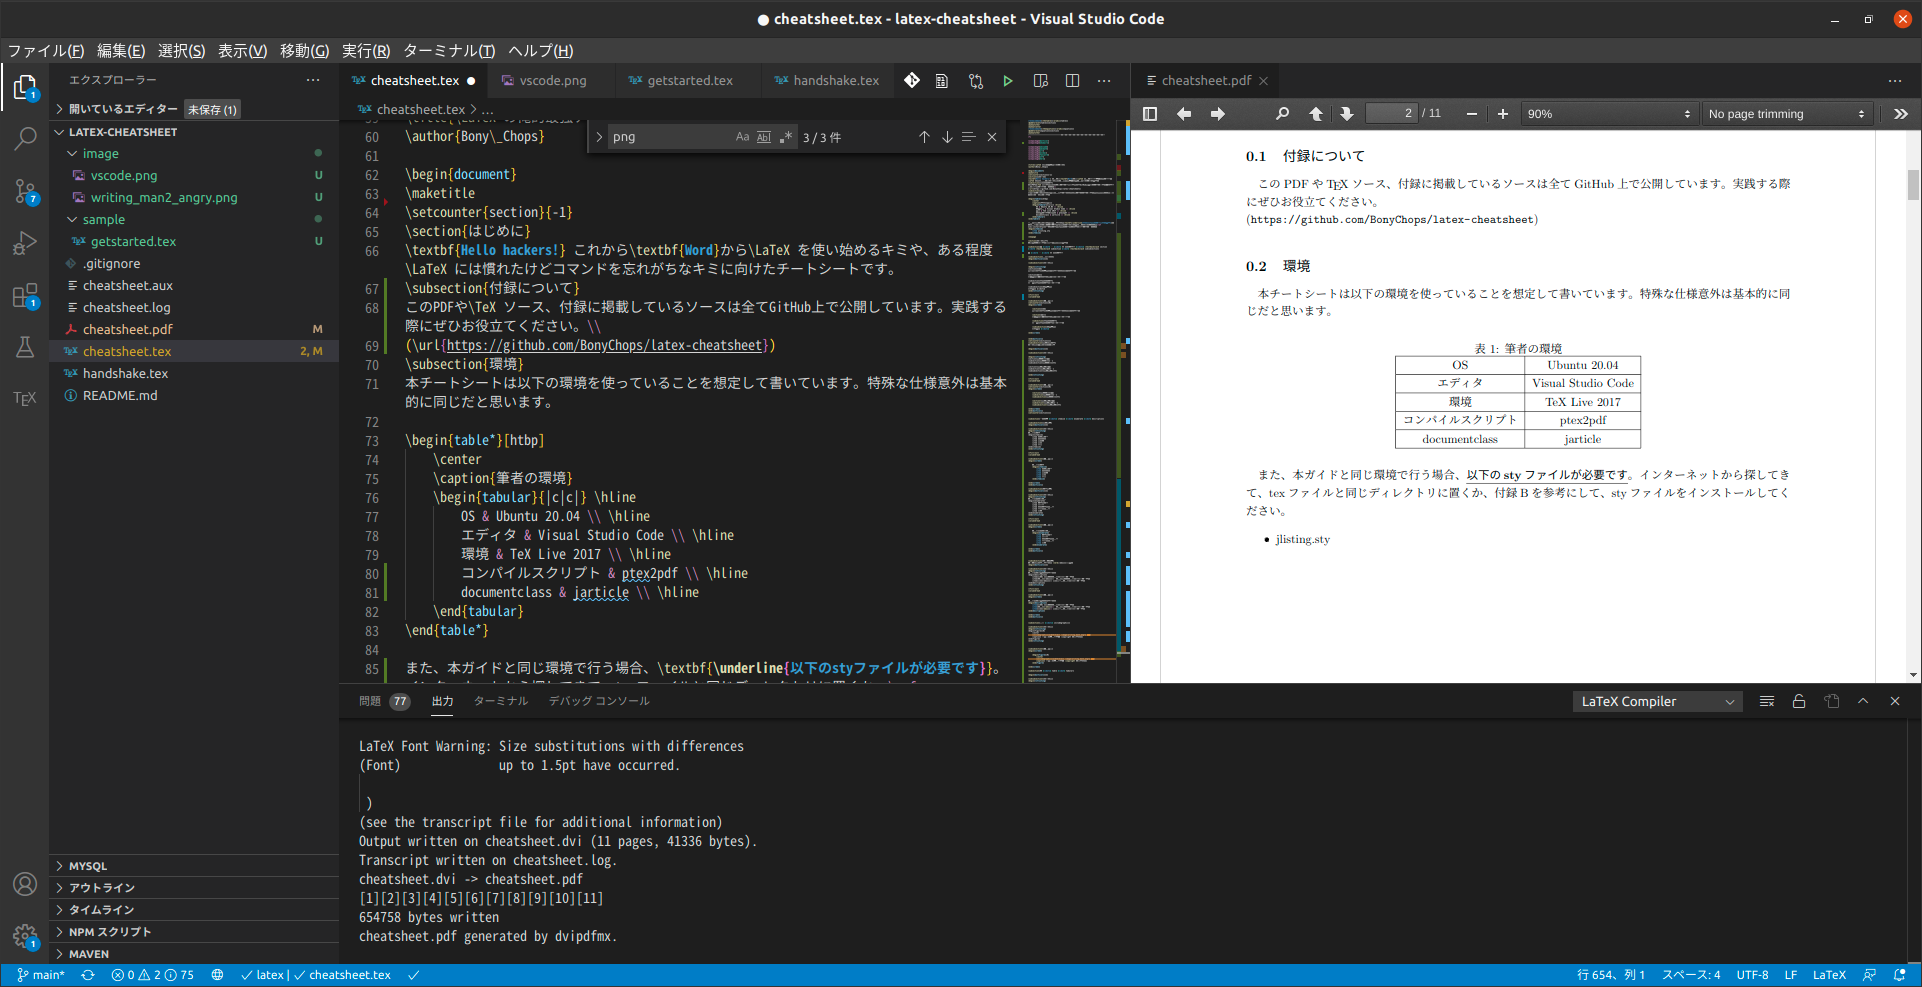
\includegraphics[width=16cm]{./image/vscode.png}
    \end{center}
\end{figure}
\TeX \ Worksと比較した時 $\cdots$
\begin{multicols*}{2}
    \subsection*{VSCodeで書くメリット}
    \begin{itemize}
        \item 複数のファイルを並べて置けるため、\textbf{PDFと\TeX ファイルを見比べながらできる!}
        \item コマンドを書く途中でサジェスト(候補)が出てくるため\textbf{すぐ書ける!間違えない!}
        \begin{figure}[H]
            \begin{center}
               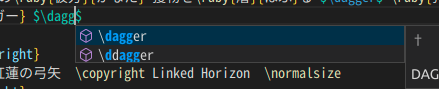
\includegraphics[width=8cm]{./image/vscode-dagger.png}
            \end{center}
        \end{figure}
        \item サイドバーにエクスプローラがあるため\textbf{複数ファイルがあっても把握しやすい!}
        \begin{figure}[H]
            \begin{center}
               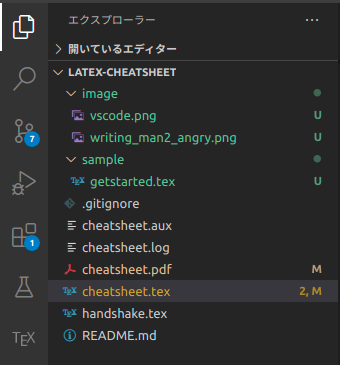
\includegraphics[width=5cm]{./image/vscode-sidebar.png}
            \end{center}
        \end{figure}
        \item エラーが(比較的)\textbf{わかりやすい!}
    \end{itemize}

\end{multicols*}

\subsection*{VSCodeで書くメリット}
\begin{itemize}
    \item a
\end{itemize}


\section{\LaTeX トラブルシューティングガイド}

\begin{thebibliography}{9}
    \bibitem{text} 令和2年度後期工学実験実習IIIテキスト
\end{thebibliography}


\end{document}